\documentclass[1p]{elsarticle_modified}
%\bibliographystyle{elsarticle-num}

%\usepackage[colorlinks]{hyperref}
%\usepackage{abbrmath_seonhwa} %\Abb, \Ascr, \Acal ,\Abf, \Afrak
\usepackage{amsfonts}
\usepackage{amssymb}
\usepackage{amsmath}
\usepackage{amsthm}
\usepackage{scalefnt}
\usepackage{amsbsy}
\usepackage{kotex}
\usepackage{caption}
\usepackage{subfig}
\usepackage{color}
\usepackage{graphicx}
\usepackage{xcolor} %% white, black, red, green, blue, cyan, magenta, yellow
\usepackage{float}
\usepackage{setspace}
\usepackage{hyperref}

\usepackage{tikz}
\usetikzlibrary{arrows}

\usepackage{multirow}
\usepackage{array} % fixed length table
\usepackage{hhline}

%%%%%%%%%%%%%%%%%%%%%
\makeatletter
\renewcommand*\env@matrix[1][\arraystretch]{%
	\edef\arraystretch{#1}%
	\hskip -\arraycolsep
	\let\@ifnextchar\new@ifnextchar
	\array{*\c@MaxMatrixCols c}}
\makeatother %https://tex.stackexchange.com/questions/14071/how-can-i-increase-the-line-spacing-in-a-matrix
%%%%%%%%%%%%%%%

\usepackage[normalem]{ulem}

\newcommand{\msout}[1]{\ifmmode\text{\sout{\ensuremath{#1}}}\else\sout{#1}\fi}
%SOURCE: \msout is \stkout macro in https://tex.stackexchange.com/questions/20609/strikeout-in-math-mode

\newcommand{\cancel}[1]{
	\ifmmode
	{\color{red}\msout{#1}}
	\else
	{\color{red}\sout{#1}}
	\fi
}

\newcommand{\add}[1]{
	{\color{blue}\uwave{#1}}
}

\newcommand{\replace}[2]{
	\ifmmode
	{\color{red}\msout{#1}}{\color{blue}\uwave{#2}}
	\else
	{\color{red}\sout{#1}}{\color{blue}\uwave{#2}}
	\fi
}

\newcommand{\Sol}{\mathcal{S}} %segment
\newcommand{\D}{D} %diagram
\newcommand{\A}{\mathcal{A}} %arc


%%%%%%%%%%%%%%%%%%%%%%%%%%%%%5 test

\def\sl{\operatorname{\textup{SL}}(2,\Cbb)}
\def\psl{\operatorname{\textup{PSL}}(2,\Cbb)}
\def\quan{\mkern 1mu \triangleright \mkern 1mu}

\theoremstyle{definition}
\newtheorem{thm}{Theorem}[section]
\newtheorem{prop}[thm]{Proposition}
\newtheorem{lem}[thm]{Lemma}
\newtheorem{ques}[thm]{Question}
\newtheorem{cor}[thm]{Corollary}
\newtheorem{defn}[thm]{Definition}
\newtheorem{exam}[thm]{Example}
\newtheorem{rmk}[thm]{Remark}
\newtheorem{alg}[thm]{Algorithm}

\newcommand{\I}{\sqrt{-1}}
\begin{document}

%\begin{frontmatter}
%
%\title{Boundary parabolic representations of knots up to 8 crossings}
%
%%% Group authors per affiliation:
%\author{Yunhi Cho} 
%\address{Department of Mathematics, University of Seoul, Seoul, Korea}
%\ead{yhcho@uos.ac.kr}
%
%
%\author{Seonhwa Kim} %\fnref{s_kim}}
%\address{Center for Geometry and Physics, Institute for Basic Science, Pohang, 37673, Korea}
%\ead{ryeona17@ibs.re.kr}
%
%\author{Hyuk Kim}
%\address{Department of Mathematical Sciences, Seoul National University, Seoul 08826, Korea}
%\ead{hyukkim@snu.ac.kr}
%
%\author{Seokbeom Yoon}
%\address{Department of Mathematical Sciences, Seoul National University, Seoul, 08826,  Korea}
%\ead{sbyoon15@snu.ac.kr}
%
%\begin{abstract}
%We find all boundary parabolic representation of knots up to 8 crossings.
%
%\end{abstract}
%\begin{keyword}
%    \MSC[2010] 57M25 
%\end{keyword}
%
%\end{frontmatter}

%\linenumbers
%\tableofcontents
%
\newcommand\colored[1]{\textcolor{white}{\rule[-0.35ex]{0.8em}{1.4ex}}\kern-0.8em\color{red} #1}%
%\newcommand\colored[1]{\textcolor{white}{ #1}\kern-2.17ex	\textcolor{white}{ #1}\kern-1.81ex	\textcolor{white}{ #1}\kern-2.15ex\color{red}#1	}

{\Large $\underline{12n_{0645}~(K12n_{0645})}$}

\setlength{\tabcolsep}{10pt}
\renewcommand{\arraystretch}{1.6}
\vspace{1cm}\begin{tabular}{m{100pt}>{\centering\arraybackslash}m{274pt}}
\multirow{5}{120pt}{
	\centering
	\includegraphics[width=112pt]{../../../GIT/diagram.site/Diagrams/png/2734_12n_0645.png}\\
\ \ \ A knot diagram\footnotemark}&
\allowdisplaybreaks
\textbf{Linearized knot diagam} \\
\cline{2-2}
 &
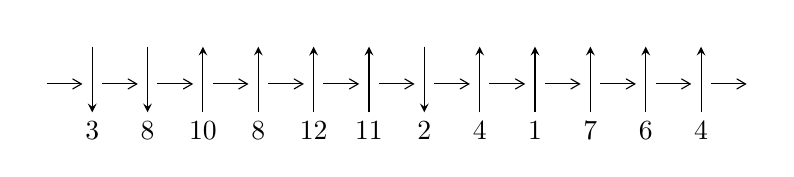
\begin{tikzpicture}[x=20pt, y=17pt]
	% nodes
	\node (C0) at (0, 0) {};
	\node (C1) at (1, 0) {};
	\node (C1U) at (1, +1) {};
	\node (C1D) at (1, -1) {3};

	\node (C2) at (2, 0) {};
	\node (C2U) at (2, +1) {};
	\node (C2D) at (2, -1) {8};

	\node (C3) at (3, 0) {};
	\node (C3U) at (3, +1) {};
	\node (C3D) at (3, -1) {10};

	\node (C4) at (4, 0) {};
	\node (C4U) at (4, +1) {};
	\node (C4D) at (4, -1) {8};

	\node (C5) at (5, 0) {};
	\node (C5U) at (5, +1) {};
	\node (C5D) at (5, -1) {12};

	\node (C6) at (6, 0) {};
	\node (C6U) at (6, +1) {};
	\node (C6D) at (6, -1) {11};

	\node (C7) at (7, 0) {};
	\node (C7U) at (7, +1) {};
	\node (C7D) at (7, -1) {2};

	\node (C8) at (8, 0) {};
	\node (C8U) at (8, +1) {};
	\node (C8D) at (8, -1) {4};

	\node (C9) at (9, 0) {};
	\node (C9U) at (9, +1) {};
	\node (C9D) at (9, -1) {1};

	\node (C10) at (10, 0) {};
	\node (C10U) at (10, +1) {};
	\node (C10D) at (10, -1) {7};

	\node (C11) at (11, 0) {};
	\node (C11U) at (11, +1) {};
	\node (C11D) at (11, -1) {6};

	\node (C12) at (12, 0) {};
	\node (C12U) at (12, +1) {};
	\node (C12D) at (12, -1) {4};
	\node (C13) at (13, 0) {};

	% arrows
	\draw[->,>={angle 60}]
	(C0) edge (C1) (C1) edge (C2) (C2) edge (C3) (C3) edge (C4) (C4) edge (C5) (C5) edge (C6) (C6) edge (C7) (C7) edge (C8) (C8) edge (C9) (C9) edge (C10) (C10) edge (C11) (C11) edge (C12) (C12) edge (C13) ;	\draw[->,>=stealth]
	(C1U) edge (C1D) (C2U) edge (C2D) (C3D) edge (C3U) (C4D) edge (C4U) (C5D) edge (C5U) (C6D) edge (C6U) (C7U) edge (C7D) (C8D) edge (C8U) (C9D) edge (C9U) (C10D) edge (C10U) (C11D) edge (C11U) (C12D) edge (C12U) ;
	\end{tikzpicture} \\
\hhline{~~} \\& 
\textbf{Solving Sequence} \\ \cline{2-2} 
 &
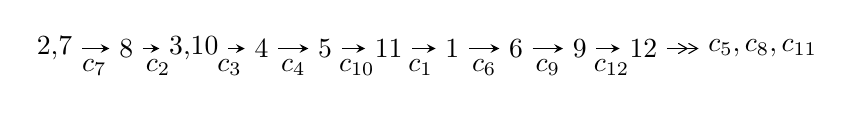
\begin{tikzpicture}[x=23pt, y=7pt]
	% node
	\node (A0) at (-1/8, 0) {2,7};
	\node (A1) at (1, 0) {8};
	\node (A2) at (33/16, 0) {3,10};
	\node (A3) at (25/8, 0) {4};
	\node (A4) at (33/8, 0) {5};
	\node (A5) at (41/8, 0) {11};
	\node (A6) at (49/8, 0) {1};
	\node (A7) at (57/8, 0) {6};
	\node (A8) at (65/8, 0) {9};
	\node (A9) at (73/8, 0) {12};
	\node (C1) at (1/2, -1) {$c_{7}$};
	\node (C2) at (3/2, -1) {$c_{2}$};
	\node (C3) at (21/8, -1) {$c_{3}$};
	\node (C4) at (29/8, -1) {$c_{4}$};
	\node (C5) at (37/8, -1) {$c_{10}$};
	\node (C6) at (45/8, -1) {$c_{1}$};
	\node (C7) at (53/8, -1) {$c_{6}$};
	\node (C8) at (61/8, -1) {$c_{9}$};
	\node (C9) at (69/8, -1) {$c_{12}$};
	\node (A10) at (11, 0) {$c_{5},c_{8},c_{11}$};

	% edge
	\draw[->,>=stealth]	
	(A0) edge (A1) (A1) edge (A2) (A2) edge (A3) (A3) edge (A4) (A4) edge (A5) (A5) edge (A6) (A6) edge (A7) (A7) edge (A8) (A8) edge (A9) ;
	\draw[->>,>={angle 60}]	
	(A9) edge (A10);
\end{tikzpicture} \\ 

\end{tabular} \\

\footnotetext{
The image of knot diagram is generated by the software ``\textbf{Draw programme}" developed by Andrew Bartholomew(\url{http://www.layer8.co.uk/maths/draw/index.htm\#Running-draw}), where we modified some parts for our purpose(\url{https://github.com/CATsTAILs/LinksPainter}).
}\phantom \\ \newline 
\centering \textbf{Ideals for irreducible components\footnotemark of $X_{\text{par}}$} 
 
\begin{align*}
I^u_{1}&=\langle 
8.90809\times10^{47} u^{45}+8.84240\times10^{47} u^{44}+\cdots+2.05702\times10^{48} b-2.45319\times10^{49},\\
\phantom{I^u_{1}}&\phantom{= \langle  }-6.59670\times10^{48} u^{45}+1.83893\times10^{49} u^{44}+\cdots+6.37677\times10^{49} a-1.07007\times10^{51},\\
\phantom{I^u_{1}}&\phantom{= \langle  }u^{46}-10 u^{44}+\cdots+11 u+31\rangle \\
I^u_{2}&=\langle 
-2 u^{10}+u^9+6 u^8-4 u^7-16 u^6+6 u^5+19 u^4-5 u^3-15 u^2+b+u+4,\\
\phantom{I^u_{2}}&\phantom{= \langle  }u^9-2 u^8-2 u^7+6 u^6+4 u^5-13 u^4-3 u^3+12 u^2+a+u-6,\\
\phantom{I^u_{2}}&\phantom{= \langle  }u^{11}- u^{10}-3 u^9+4 u^8+7 u^7-8 u^6-8 u^5+9 u^4+5 u^3-5 u^2- u+1\rangle \\
\\
\end{align*}
\raggedright * 2 irreducible components of $\dim_{\mathbb{C}}=0$, with total 57 representations.\\
\footnotetext{All coefficients of polynomials are rational numbers. But the coefficients are sometimes approximated in decimal forms when there is not enough margin.}
\newpage
\renewcommand{\arraystretch}{1}
\centering \section*{I. $I^u_{1}= \langle 8.91\times10^{47} u^{45}+8.84\times10^{47} u^{44}+\cdots+2.06\times10^{48} b-2.45\times10^{49},\;-6.60\times10^{48} u^{45}+1.84\times10^{49} u^{44}+\cdots+6.38\times10^{49} a-1.07\times10^{51},\;u^{46}-10 u^{44}+\cdots+11 u+31 \rangle$}
\flushleft \textbf{(i) Arc colorings}\\
\begin{tabular}{m{7pt} m{180pt} m{7pt} m{180pt} }
\flushright $a_{2}=$&$\begin{pmatrix}0\\u\end{pmatrix}$ \\
\flushright $a_{7}=$&$\begin{pmatrix}1\\0\end{pmatrix}$ \\
\flushright $a_{8}=$&$\begin{pmatrix}1\\u^2\end{pmatrix}$ \\
\flushright $a_{3}=$&$\begin{pmatrix}- u\\- u^3+u\end{pmatrix}$ \\
\flushright $a_{10}=$&$\begin{pmatrix}0.103449 u^{45}-0.288379 u^{44}+\cdots-0.284809 u+16.7807\\-0.433057 u^{45}-0.429864 u^{44}+\cdots+15.8856 u+11.9259\end{pmatrix}$ \\
\flushright $a_{4}=$&$\begin{pmatrix}-0.141416 u^{45}+0.395932 u^{44}+\cdots-9.32244 u-28.9599\\0.366395 u^{45}+0.483053 u^{44}+\cdots-16.9943 u-16.7074\end{pmatrix}$ \\
\flushright $a_{5}=$&$\begin{pmatrix}0.284534 u^{45}+0.603944 u^{44}+\cdots-26.3454 u-33.3933\\0.611972 u^{45}+0.566589 u^{44}+\cdots-32.4869 u-23.1557\end{pmatrix}$ \\
\flushright $a_{11}=$&$\begin{pmatrix}-0.329608 u^{45}-0.718243 u^{44}+\cdots+15.6007 u+28.7066\\-0.433057 u^{45}-0.429864 u^{44}+\cdots+15.8856 u+11.9259\end{pmatrix}$ \\
\flushright $a_{1}=$&$\begin{pmatrix}u^3\\u^5- u^3+u\end{pmatrix}$ \\
\flushright $a_{6}=$&$\begin{pmatrix}1.30358 u^{45}+0.927847 u^{44}+\cdots-65.6458 u-32.8545\\0.264798 u^{45}+0.224989 u^{44}+\cdots-12.0873 u-7.10220\end{pmatrix}$ \\
\flushright $a_{9}=$&$\begin{pmatrix}0.365076 u^{45}-0.0975018 u^{44}+\cdots-13.4315 u+10.4704\\-0.146690 u^{45}-0.269810 u^{44}+\cdots+2.05043 u+6.63521\end{pmatrix}$ \\
\flushright $a_{12}=$&$\begin{pmatrix}1.08634 u^{45}+0.507925 u^{44}+\cdots-43.7616 u-12.5340\\1.02109 u^{45}+0.771426 u^{44}+\cdots-46.8793 u-30.5007\end{pmatrix}$\\&\end{tabular}
\flushleft \textbf{(ii) Obstruction class $= -1$}\\~\\
\flushleft \textbf{(iii) Cusp Shapes $= -0.400585 u^{45}-0.275909 u^{44}+\cdots-48.1051 u-42.5676$}\\~\\
\newpage\renewcommand{\arraystretch}{1}
\flushleft \textbf{(iv) u-Polynomials at the component}\newline \\
\begin{tabular}{m{50pt}|m{274pt}}
Crossings & \hspace{64pt}u-Polynomials at each crossing \\
\hline $$\begin{aligned}c_{1}\end{aligned}$$&$\begin{aligned}
&u^{46}+20 u^{45}+\cdots+14009 u+961
\end{aligned}$\\
\hline $$\begin{aligned}c_{2},c_{7}\end{aligned}$$&$\begin{aligned}
&u^{46}-10 u^{44}+\cdots-11 u+31
\end{aligned}$\\
\hline $$\begin{aligned}c_{3}\end{aligned}$$&$\begin{aligned}
&u^{46}+u^{45}+\cdots+2 u-1
\end{aligned}$\\
\hline $$\begin{aligned}c_{4},c_{8}\end{aligned}$$&$\begin{aligned}
&u^{46}-3 u^{45}+\cdots-2160 u-1621
\end{aligned}$\\
\hline $$\begin{aligned}c_{5},c_{6},c_{10}\\c_{11}\end{aligned}$$&$\begin{aligned}
&u^{46}- u^{45}+\cdots-10 u-1
\end{aligned}$\\
\hline $$\begin{aligned}c_{9}\end{aligned}$$&$\begin{aligned}
&u^{46}-24 u^{44}+\cdots+183 u+43
\end{aligned}$\\
\hline $$\begin{aligned}c_{12}\end{aligned}$$&$\begin{aligned}
&u^{46}+7 u^{45}+\cdots-3420 u-343
\end{aligned}$\\
\hline
\end{tabular}\\~\\
\newpage\renewcommand{\arraystretch}{1}
\flushleft \textbf{(v) Riley Polynomials at the component}\newline \\
\begin{tabular}{m{50pt}|m{274pt}}
Crossings & \hspace{64pt}Riley Polynomials at each crossing \\
\hline $$\begin{aligned}c_{1}\end{aligned}$$&$\begin{aligned}
&y^{46}+32 y^{45}+\cdots+2013751 y+923521
\end{aligned}$\\
\hline $$\begin{aligned}c_{2},c_{7}\end{aligned}$$&$\begin{aligned}
&y^{46}-20 y^{45}+\cdots-14009 y+961
\end{aligned}$\\
\hline $$\begin{aligned}c_{3}\end{aligned}$$&$\begin{aligned}
&y^{46}+7 y^{45}+\cdots-42 y+1
\end{aligned}$\\
\hline $$\begin{aligned}c_{4},c_{8}\end{aligned}$$&$\begin{aligned}
&y^{46}-41 y^{45}+\cdots-68296334 y+2627641
\end{aligned}$\\
\hline $$\begin{aligned}c_{5},c_{6},c_{10}\\c_{11}\end{aligned}$$&$\begin{aligned}
&y^{46}+51 y^{45}+\cdots-60 y+1
\end{aligned}$\\
\hline $$\begin{aligned}c_{9}\end{aligned}$$&$\begin{aligned}
&y^{46}-48 y^{45}+\cdots-93001 y+1849
\end{aligned}$\\
\hline $$\begin{aligned}c_{12}\end{aligned}$$&$\begin{aligned}
&y^{46}-51 y^{45}+\cdots-4953020 y+117649
\end{aligned}$\\
\hline
\end{tabular}\\~\\
\newpage\flushleft \textbf{(vi) Complex Volumes and Cusp Shapes}
$$\begin{array}{c|c|c}  
\text{Solutions to }I^u_{1}& \I (\text{vol} + \sqrt{-1}CS) & \text{Cusp shape}\\
 \hline 
\begin{aligned}
u &= \phantom{-}0.777171 + 0.612835 I \\
a &= \phantom{-}1.016300 - 0.099619 I \\
b &= -0.331933 + 0.632697 I\end{aligned}
 & -0.45486 - 2.22136 I & \phantom{-}5.56372 + 4.55995 I \\ \hline\begin{aligned}
u &= \phantom{-}0.777171 - 0.612835 I \\
a &= \phantom{-}1.016300 + 0.099619 I \\
b &= -0.331933 - 0.632697 I\end{aligned}
 & -0.45486 + 2.22136 I & \phantom{-}5.56372 - 4.55995 I \\ \hline\begin{aligned}
u &= -0.796260 + 0.581104 I \\
a &= \phantom{-}0.123978 - 0.214987 I \\
b &= -0.37211 + 1.50267 I\end{aligned}
 & -0.132688 - 0.463216 I & \phantom{-}4.30646 - 2.07954 I \\ \hline\begin{aligned}
u &= -0.796260 - 0.581104 I \\
a &= \phantom{-}0.123978 + 0.214987 I \\
b &= -0.37211 - 1.50267 I\end{aligned}
 & -0.132688 + 0.463216 I & \phantom{-}4.30646 + 2.07954 I \\ \hline\begin{aligned}
u &= \phantom{-}0.891195 + 0.365209 I \\
a &= \phantom{-}2.81275 + 0.31631 I \\
b &= \phantom{-}0.031259 + 1.382470 I\end{aligned}
 & -1.86336 + 0.58097 I & \phantom{-}3.38443 + 0.69263 I \\ \hline\begin{aligned}
u &= \phantom{-}0.891195 - 0.365209 I \\
a &= \phantom{-}2.81275 - 0.31631 I \\
b &= \phantom{-}0.031259 - 1.382470 I\end{aligned}
 & -1.86336 - 0.58097 I & \phantom{-}3.38443 - 0.69263 I \\ \hline\begin{aligned}
u &= \phantom{-}0.758477 + 0.770111 I \\
a &= -1.31515 - 0.65871 I \\
b &= \phantom{-}0.712311 - 0.622242 I\end{aligned}
 & \phantom{-}6.85172 - 1.46852 I & \phantom{-}7.65009 + 3.31921 I \\ \hline\begin{aligned}
u &= \phantom{-}0.758477 - 0.770111 I \\
a &= -1.31515 + 0.65871 I \\
b &= \phantom{-}0.712311 + 0.622242 I\end{aligned}
 & \phantom{-}6.85172 + 1.46852 I & \phantom{-}7.65009 - 3.31921 I \\ \hline\begin{aligned}
u &= -0.913123 + 0.579538 I \\
a &= -1.81688 + 0.86698 I \\
b &= \phantom{-}0.25012 + 1.59325 I\end{aligned}
 & -0.51224 + 5.07727 I & \phantom{-}3.91334 - 4.47739 I \\ \hline\begin{aligned}
u &= -0.913123 - 0.579538 I \\
a &= -1.81688 - 0.86698 I \\
b &= \phantom{-}0.25012 - 1.59325 I\end{aligned}
 & -0.51224 - 5.07727 I & \phantom{-}3.91334 + 4.47739 I\\
 \hline 
 \end{array}$$\newpage$$\begin{array}{c|c|c}  
\text{Solutions to }I^u_{1}& \I (\text{vol} + \sqrt{-1}CS) & \text{Cusp shape}\\
 \hline 
\begin{aligned}
u &= \phantom{-}0.913895 + 0.666325 I \\
a &= -0.649069 + 0.227447 I \\
b &= \phantom{-}0.338025 - 0.053987 I\end{aligned}
 & -1.08476 - 2.74841 I & \phantom{-}8.58326 + 2.30981 I \\ \hline\begin{aligned}
u &= \phantom{-}0.913895 - 0.666325 I \\
a &= -0.649069 - 0.227447 I \\
b &= \phantom{-}0.338025 + 0.053987 I\end{aligned}
 & -1.08476 + 2.74841 I & \phantom{-}8.58326 - 2.30981 I \\ \hline\begin{aligned}
u &= \phantom{-}0.854412 + 0.074876 I \\
a &= -0.93971 - 1.27956 I \\
b &= \phantom{-}0.02815 - 1.72557 I\end{aligned}
 & -13.22450 - 0.32397 I & -0.99400 - 2.11493 I \\ \hline\begin{aligned}
u &= \phantom{-}0.854412 - 0.074876 I \\
a &= -0.93971 + 1.27956 I \\
b &= \phantom{-}0.02815 + 1.72557 I\end{aligned}
 & -13.22450 + 0.32397 I & -0.99400 + 2.11493 I \\ \hline\begin{aligned}
u &= \phantom{-}0.812024 + 0.266747 I \\
a &= \phantom{-}1.03314 - 1.16176 I \\
b &= -0.222226 + 1.219740 I\end{aligned}
 & -1.58775 - 3.40530 I & \phantom{-}2.42508 + 8.01994 I \\ \hline\begin{aligned}
u &= \phantom{-}0.812024 - 0.266747 I \\
a &= \phantom{-}1.03314 + 1.16176 I \\
b &= -0.222226 - 1.219740 I\end{aligned}
 & -1.58775 + 3.40530 I & \phantom{-}2.42508 - 8.01994 I \\ \hline\begin{aligned}
u &= -0.612129 + 0.975994 I \\
a &= -0.737727 + 0.580195 I \\
b &= \phantom{-}0.741768 - 0.448363 I\end{aligned}
 & \phantom{-}7.36473 - 3.39333 I & \phantom{-}8.53065 + 3.23087 I \\ \hline\begin{aligned}
u &= -0.612129 - 0.975994 I \\
a &= -0.737727 - 0.580195 I \\
b &= \phantom{-}0.741768 + 0.448363 I\end{aligned}
 & \phantom{-}7.36473 + 3.39333 I & \phantom{-}8.53065 - 3.23087 I \\ \hline\begin{aligned}
u &= \phantom{-}0.066989 + 0.834868 I \\
a &= \phantom{-}0.507773 + 0.449914 I \\
b &= -0.081495 - 1.363900 I\end{aligned}
 & -3.81447 + 2.16547 I & \phantom{-}3.03202 - 3.16202 I \\ \hline\begin{aligned}
u &= \phantom{-}0.066989 - 0.834868 I \\
a &= \phantom{-}0.507773 - 0.449914 I \\
b &= -0.081495 + 1.363900 I\end{aligned}
 & -3.81447 - 2.16547 I & \phantom{-}3.03202 + 3.16202 I\\
 \hline 
 \end{array}$$\newpage$$\begin{array}{c|c|c}  
\text{Solutions to }I^u_{1}& \I (\text{vol} + \sqrt{-1}CS) & \text{Cusp shape}\\
 \hline 
\begin{aligned}
u &= -0.835340\phantom{ +0.000000I} \\
a &= \phantom{-}1.52762\phantom{ +0.000000I} \\
b &= -0.699978\phantom{ +0.000000I}\end{aligned}
 & \phantom{-}2.08624\phantom{ +0.000000I} & \phantom{-}3.59250\phantom{ +0.000000I} \\ \hline\begin{aligned}
u &= \phantom{-}0.957184 + 0.700082 I \\
a &= \phantom{-}0.757512 + 0.366942 I \\
b &= -0.873917 - 0.486869 I\end{aligned}
 & \phantom{-}6.22467 - 4.09819 I & \phantom{-}6.87161 + 2.72251 I \\ \hline\begin{aligned}
u &= \phantom{-}0.957184 - 0.700082 I \\
a &= \phantom{-}0.757512 - 0.366942 I \\
b &= -0.873917 + 0.486869 I\end{aligned}
 & \phantom{-}6.22467 + 4.09819 I & \phantom{-}6.87161 - 2.72251 I \\ \hline\begin{aligned}
u &= -1.077260 + 0.505176 I \\
a &= -1.068580 + 0.594060 I \\
b &= \phantom{-}0.485546 + 0.365826 I\end{aligned}
 & -1.04957 + 4.66742 I & \phantom{-}5.56090 - 9.70253 I \\ \hline\begin{aligned}
u &= -1.077260 - 0.505176 I \\
a &= -1.068580 - 0.594060 I \\
b &= \phantom{-}0.485546 - 0.365826 I\end{aligned}
 & -1.04957 - 4.66742 I & \phantom{-}5.56090 + 9.70253 I \\ \hline\begin{aligned}
u &= \phantom{-}1.152890 + 0.432401 I \\
a &= -0.0608762 - 0.0298599 I \\
b &= \phantom{-}0.057001 + 0.488154 I\end{aligned}
 & -1.61761 - 2.37559 I & \phantom{-}0.879006 + 0.401607 I \\ \hline\begin{aligned}
u &= \phantom{-}1.152890 - 0.432401 I \\
a &= -0.0608762 + 0.0298599 I \\
b &= \phantom{-}0.057001 - 0.488154 I\end{aligned}
 & -1.61761 + 2.37559 I & \phantom{-}0.879006 - 0.401607 I \\ \hline\begin{aligned}
u &= -0.708951 + 0.204573 I \\
a &= -0.837428 - 0.839652 I \\
b &= \phantom{-}0.231335 - 0.896256 I\end{aligned}
 & -3.73770 + 0.61521 I & -1.20649 + 1.42032 I \\ \hline\begin{aligned}
u &= -0.708951 - 0.204573 I \\
a &= -0.837428 + 0.839652 I \\
b &= \phantom{-}0.231335 + 0.896256 I\end{aligned}
 & -3.73770 - 0.61521 I & -1.20649 - 1.42032 I \\ \hline\begin{aligned}
u &= \phantom{-}0.474202 + 1.186570 I \\
a &= -0.207177 - 0.587661 I \\
b &= \phantom{-}0.25018 + 1.48994 I\end{aligned}
 & \phantom{-}1.08764 + 6.97219 I & \phantom{-}4.72387 - 4.64542 I\\
 \hline 
 \end{array}$$\newpage$$\begin{array}{c|c|c}  
\text{Solutions to }I^u_{1}& \I (\text{vol} + \sqrt{-1}CS) & \text{Cusp shape}\\
 \hline 
\begin{aligned}
u &= \phantom{-}0.474202 - 1.186570 I \\
a &= -0.207177 + 0.587661 I \\
b &= \phantom{-}0.25018 - 1.48994 I\end{aligned}
 & \phantom{-}1.08764 - 6.97219 I & \phantom{-}4.72387 + 4.64542 I \\ \hline\begin{aligned}
u &= -0.713380\phantom{ +0.000000I} \\
a &= \phantom{-}3.04004\phantom{ +0.000000I} \\
b &= \phantom{-}0.136531\phantom{ +0.000000I}\end{aligned}
 & \phantom{-}2.80045\phantom{ +0.000000I} & -4.62300\phantom{ +0.000000I} \\ \hline\begin{aligned}
u &= \phantom{-}1.195490 + 0.523779 I \\
a &= -1.69838 - 0.65171 I \\
b &= \phantom{-}0.16723 - 1.46549 I\end{aligned}
 & -7.05077 - 7.05212 I & \phantom{-}1.18080 + 6.79998 I \\ \hline\begin{aligned}
u &= \phantom{-}1.195490 - 0.523779 I \\
a &= -1.69838 + 0.65171 I \\
b &= \phantom{-}0.16723 + 1.46549 I\end{aligned}
 & -7.05077 + 7.05212 I & \phantom{-}1.18080 - 6.79998 I \\ \hline\begin{aligned}
u &= -1.097350 + 0.743718 I \\
a &= \phantom{-}1.174780 - 0.336310 I \\
b &= -0.817170 - 0.613699 I\end{aligned}
 & \phantom{-}5.83564 + 9.64943 I & \phantom{-}6.00000 - 7.00268 I \\ \hline\begin{aligned}
u &= -1.097350 - 0.743718 I \\
a &= \phantom{-}1.174780 + 0.336310 I \\
b &= -0.817170 + 0.613699 I\end{aligned}
 & \phantom{-}5.83564 - 9.64943 I & \phantom{-}6.00000 + 7.00268 I \\ \hline\begin{aligned}
u &= -0.378903 + 0.518753 I \\
a &= \phantom{-}1.067570 - 0.111522 I \\
b &= -0.441328 + 0.176398 I\end{aligned}
 & \phantom{-}0.963425 - 0.418051 I & \phantom{-}9.96672 + 3.30631 I \\ \hline\begin{aligned}
u &= -0.378903 - 0.518753 I \\
a &= \phantom{-}1.067570 + 0.111522 I \\
b &= -0.441328 - 0.176398 I\end{aligned}
 & \phantom{-}0.963425 + 0.418051 I & \phantom{-}9.96672 - 3.30631 I \\ \hline\begin{aligned}
u &= -1.130590 + 0.839549 I \\
a &= \phantom{-}0.972367 + 0.073701 I \\
b &= -0.09034 - 1.57331 I\end{aligned}
 & -7.92848 + 3.74029 I & \phantom{-0.000000 } 0 \\ \hline\begin{aligned}
u &= -1.130590 - 0.839549 I \\
a &= \phantom{-}0.972367 - 0.073701 I \\
b &= -0.09034 + 1.57331 I\end{aligned}
 & -7.92848 - 3.74029 I & \phantom{-0.000000 } 0\\
 \hline 
 \end{array}$$\newpage$$\begin{array}{c|c|c}  
\text{Solutions to }I^u_{1}& \I (\text{vol} + \sqrt{-1}CS) & \text{Cusp shape}\\
 \hline 
\begin{aligned}
u &= \phantom{-}1.22337 + 0.74620 I \\
a &= \phantom{-}1.47635 + 0.22540 I \\
b &= -0.28946 + 1.57516 I\end{aligned}
 & -1.32243 - 13.76490 I & \phantom{-0.000000 } 0 \\ \hline\begin{aligned}
u &= \phantom{-}1.22337 - 0.74620 I \\
a &= \phantom{-}1.47635 - 0.22540 I \\
b &= -0.28946 - 1.57516 I\end{aligned}
 & -1.32243 + 13.76490 I & \phantom{-0.000000 } 0 \\ \hline\begin{aligned}
u &= -1.12014 + 0.96904 I \\
a &= -0.842997 - 0.382179 I \\
b &= \phantom{-}0.060969 + 1.402580 I\end{aligned}
 & -5.91695 + 3.87147 I & \phantom{-0.000000 } 0 \\ \hline\begin{aligned}
u &= -1.12014 - 0.96904 I \\
a &= -0.842997 + 0.382179 I \\
b &= \phantom{-}0.060969 - 1.402580 I\end{aligned}
 & -5.91695 - 3.87147 I & \phantom{-0.000000 } 0 \\ \hline\begin{aligned}
u &= -1.46824 + 0.34467 I \\
a &= \phantom{-}0.350849 - 0.635636 I \\
b &= -0.05218 - 1.50558 I\end{aligned}
 & -8.25938 + 2.77632 I & \phantom{-0.000000 } 0 \\ \hline\begin{aligned}
u &= -1.46824 - 0.34467 I \\
a &= \phantom{-}0.350849 + 0.635636 I \\
b &= -0.05218 + 1.50558 I\end{aligned}
 & -8.25938 - 2.77632 I & \phantom{-0.000000 } 0\\
 \hline 
 \end{array}$$\newpage\newpage\renewcommand{\arraystretch}{1}
\centering \section*{II. $I^u_{2}= \langle -2 u^{10}+u^9+\cdots+b+4,\;u^9-2 u^8+\cdots+a-6,\;u^{11}- u^{10}+\cdots- u+1 \rangle$}
\flushleft \textbf{(i) Arc colorings}\\
\begin{tabular}{m{7pt} m{180pt} m{7pt} m{180pt} }
\flushright $a_{2}=$&$\begin{pmatrix}0\\u\end{pmatrix}$ \\
\flushright $a_{7}=$&$\begin{pmatrix}1\\0\end{pmatrix}$ \\
\flushright $a_{8}=$&$\begin{pmatrix}1\\u^2\end{pmatrix}$ \\
\flushright $a_{3}=$&$\begin{pmatrix}- u\\- u^3+u\end{pmatrix}$ \\
\flushright $a_{10}=$&$\begin{pmatrix}- u^9+2 u^8+2 u^7-6 u^6-4 u^5+13 u^4+3 u^3-12 u^2- u+6\\2 u^{10}- u^9-6 u^8+4 u^7+16 u^6-6 u^5-19 u^4+5 u^3+15 u^2- u-4\end{pmatrix}$ \\
\flushright $a_{4}=$&$\begin{pmatrix}- u^{10}+4 u^9-11 u^7+3 u^6+24 u^5-9 u^4-22 u^3+10 u^2+9 u-3\\u^{10}+u^9-5 u^8- u^7+14 u^6+3 u^5-20 u^4-2 u^3+16 u^2-4\end{pmatrix}$ \\
\flushright $a_{5}=$&$\begin{pmatrix}3 u^9-3 u^8-7 u^7+10 u^6+16 u^5-17 u^4-13 u^3+15 u^2+5 u-4\\u^{10}+u^9-5 u^8- u^7+14 u^6+3 u^5-20 u^4- u^3+16 u^2- u-4\end{pmatrix}$ \\
\flushright $a_{11}=$&$\begin{pmatrix}2 u^{10}-2 u^9-4 u^8+6 u^7+10 u^6-10 u^5-6 u^4+8 u^3+3 u^2-2 u+2\\2 u^{10}- u^9-6 u^8+4 u^7+16 u^6-6 u^5-19 u^4+5 u^3+15 u^2- u-4\end{pmatrix}$ \\
\flushright $a_{1}=$&$\begin{pmatrix}u^3\\u^5- u^3+u\end{pmatrix}$ \\
\flushright $a_{6}=$&$\begin{pmatrix}7 u^{10}-5 u^9+\cdots-7 u-8\\-2 u^9+2 u^8+5 u^7-7 u^6-11 u^5+12 u^4+10 u^3-11 u^2-4 u+2\end{pmatrix}$ \\
\flushright $a_{9}=$&$\begin{pmatrix}- u^9+2 u^8+2 u^7-6 u^6-4 u^5+13 u^4+3 u^3-11 u^2- u+6\\2 u^{10}- u^9-6 u^8+4 u^7+16 u^6-6 u^5-18 u^4+5 u^3+14 u^2- u-3\end{pmatrix}$ \\
\flushright $a_{12}=$&$\begin{pmatrix}-2 u^9+u^8+7 u^7-6 u^6-16 u^5+10 u^4+19 u^3-12 u^2-9 u+4\\-2 u^{10}+2 u^9+\cdots+3 u+3\end{pmatrix}$\\&\end{tabular}
\flushleft \textbf{(ii) Obstruction class $= 1$}\\~\\
\flushleft \textbf{(iii) Cusp Shapes $= 8 u^{10}-13 u^9-14 u^8+40 u^7+26 u^6-77 u^5-2 u^4+70 u^3-13 u^2-28 u+15$}\\~\\
\newpage\renewcommand{\arraystretch}{1}
\flushleft \textbf{(iv) u-Polynomials at the component}\newline \\
\begin{tabular}{m{50pt}|m{274pt}}
Crossings & \hspace{64pt}u-Polynomials at each crossing \\
\hline $$\begin{aligned}c_{1}\end{aligned}$$&$\begin{aligned}
&u^{11}-7 u^{10}+\cdots+11 u-1
\end{aligned}$\\
\hline $$\begin{aligned}c_{2}\end{aligned}$$&$\begin{aligned}
&u^{11}+u^{10}-3 u^9-4 u^8+7 u^7+8 u^6-8 u^5-9 u^4+5 u^3+5 u^2- u-1
\end{aligned}$\\
\hline $$\begin{aligned}c_{3}\end{aligned}$$&$\begin{aligned}
&u^{11}+4 u^9+u^8+3 u^7- u^5-3 u^4- u^3-2 u^2-1
\end{aligned}$\\
\hline $$\begin{aligned}c_{4}\end{aligned}$$&$\begin{aligned}
&u^{11}+2 u^9- u^8+3 u^7- u^6+3 u^4- u^3+4 u^2+1
\end{aligned}$\\
\hline $$\begin{aligned}c_{5},c_{6}\end{aligned}$$&$\begin{aligned}
&u^{11}+8 u^9+23 u^7+28 u^5+u^4+12 u^3+3 u^2+1
\end{aligned}$\\
\hline $$\begin{aligned}c_{7}\end{aligned}$$&$\begin{aligned}
&u^{11}- u^{10}-3 u^9+4 u^8+7 u^7-8 u^6-8 u^5+9 u^4+5 u^3-5 u^2- u+1
\end{aligned}$\\
\hline $$\begin{aligned}c_{8}\end{aligned}$$&$\begin{aligned}
&u^{11}+2 u^9+u^8+3 u^7+u^6-3 u^4- u^3-4 u^2-1
\end{aligned}$\\
\hline $$\begin{aligned}c_{9}\end{aligned}$$&$\begin{aligned}
&u^{11}- u^{10}-5 u^9+5 u^8+9 u^7-8 u^6-8 u^5+7 u^4+4 u^3-3 u^2- u+1
\end{aligned}$\\
\hline $$\begin{aligned}c_{10},c_{11}\end{aligned}$$&$\begin{aligned}
&u^{11}+8 u^9+23 u^7+28 u^5- u^4+12 u^3-3 u^2-1
\end{aligned}$\\
\hline $$\begin{aligned}c_{12}\end{aligned}$$&$\begin{aligned}
&u^{11}+3 u^9+8 u^8+3 u^7+10 u^6+12 u^5+u^4+9 u^3+5 u^2-4 u+1
\end{aligned}$\\
\hline
\end{tabular}\\~\\
\newpage\renewcommand{\arraystretch}{1}
\flushleft \textbf{(v) Riley Polynomials at the component}\newline \\
\begin{tabular}{m{50pt}|m{274pt}}
Crossings & \hspace{64pt}Riley Polynomials at each crossing \\
\hline $$\begin{aligned}c_{1}\end{aligned}$$&$\begin{aligned}
&y^{11}+13 y^{10}+\cdots+15 y-1
\end{aligned}$\\
\hline $$\begin{aligned}c_{2},c_{7}\end{aligned}$$&$\begin{aligned}
&y^{11}-7 y^{10}+\cdots+11 y-1
\end{aligned}$\\
\hline $$\begin{aligned}c_{3}\end{aligned}$$&$\begin{aligned}
&y^{11}+8 y^{10}+\cdots-4 y-1
\end{aligned}$\\
\hline $$\begin{aligned}c_{4},c_{8}\end{aligned}$$&$\begin{aligned}
&y^{11}+4 y^{10}+\cdots-8 y-1
\end{aligned}$\\
\hline $$\begin{aligned}c_{5},c_{6},c_{10}\\c_{11}\end{aligned}$$&$\begin{aligned}
&y^{11}+16 y^{10}+\cdots-6 y-1
\end{aligned}$\\
\hline $$\begin{aligned}c_{9}\end{aligned}$$&$\begin{aligned}
&y^{11}-11 y^{10}+\cdots+7 y-1
\end{aligned}$\\
\hline $$\begin{aligned}c_{12}\end{aligned}$$&$\begin{aligned}
&y^{11}+6 y^{10}+\cdots+6 y-1
\end{aligned}$\\
\hline
\end{tabular}\\~\\
\newpage\flushleft \textbf{(vi) Complex Volumes and Cusp Shapes}
$$\begin{array}{c|c|c}  
\text{Solutions to }I^u_{2}& \I (\text{vol} + \sqrt{-1}CS) & \text{Cusp shape}\\
 \hline 
\begin{aligned}
u &= -0.926350 + 0.275446 I \\
a &= \phantom{-}0.604065 - 1.072750 I \\
b &= \phantom{-}0.02836 - 1.73242 I\end{aligned}
 & -13.09290 + 1.15540 I & \phantom{-}1.12930 - 6.75991 I \\ \hline\begin{aligned}
u &= -0.926350 - 0.275446 I \\
a &= \phantom{-}0.604065 + 1.072750 I \\
b &= \phantom{-}0.02836 + 1.73242 I\end{aligned}
 & -13.09290 - 1.15540 I & \phantom{-}1.12930 + 6.75991 I \\ \hline\begin{aligned}
u &= \phantom{-}0.931716 + 0.451527 I \\
a &= -0.012829 + 0.293025 I \\
b &= \phantom{-}0.166908 + 0.916041 I\end{aligned}
 & -3.41093 - 1.89765 I & \phantom{-}0.48715 + 3.11270 I \\ \hline\begin{aligned}
u &= \phantom{-}0.931716 - 0.451527 I \\
a &= -0.012829 - 0.293025 I \\
b &= \phantom{-}0.166908 - 0.916041 I\end{aligned}
 & -3.41093 + 1.89765 I & \phantom{-}0.48715 - 3.11270 I \\ \hline\begin{aligned}
u &= -1.092600 + 0.709214 I \\
a &= -0.636248 - 0.082249 I \\
b &= \phantom{-}0.193075 + 0.390923 I\end{aligned}
 & -1.63003 + 3.19570 I & -1.52279 - 9.85073 I \\ \hline\begin{aligned}
u &= -1.092600 - 0.709214 I \\
a &= -0.636248 + 0.082249 I \\
b &= \phantom{-}0.193075 - 0.390923 I\end{aligned}
 & -1.63003 - 3.19570 I & -1.52279 + 9.85073 I \\ \hline\begin{aligned}
u &= \phantom{-}0.605049 + 0.142384 I \\
a &= \phantom{-}2.74610 - 0.77777 I \\
b &= -0.233007 + 1.358440 I\end{aligned}
 & -1.39419 - 2.51034 I & \phantom{-}3.76451 + 0.24190 I \\ \hline\begin{aligned}
u &= \phantom{-}0.605049 - 0.142384 I \\
a &= \phantom{-}2.74610 + 0.77777 I \\
b &= -0.233007 - 1.358440 I\end{aligned}
 & -1.39419 + 2.51034 I & \phantom{-}3.76451 - 0.24190 I \\ \hline\begin{aligned}
u &= -0.612040\phantom{ +0.000000I} \\
a &= \phantom{-}3.26852\phantom{ +0.000000I} \\
b &= -0.445195\phantom{ +0.000000I}\end{aligned}
 & \phantom{-}3.18891\phantom{ +0.000000I} & \phantom{-}17.5710\phantom{ +0.000000I} \\ \hline\begin{aligned}
u &= \phantom{-}1.28821 + 0.91096 I \\
a &= -0.835352 + 0.045091 I \\
b &= \phantom{-}0.06726 - 1.54442 I\end{aligned}
 & -8.38532 - 4.16451 I & -4.14359 + 8.28004 I\\
 \hline 
 \end{array}$$\newpage$$\begin{array}{c|c|c}  
\text{Solutions to }I^u_{2}& \I (\text{vol} + \sqrt{-1}CS) & \text{Cusp shape}\\
 \hline 
\begin{aligned}
u &= \phantom{-}1.28821 - 0.91096 I \\
a &= -0.835352 - 0.045091 I \\
b &= \phantom{-}0.06726 + 1.54442 I\end{aligned}
 & -8.38532 + 4.16451 I & -4.14359 - 8.28004 I\\
 \hline 
 \end{array}$$\newpage
\newpage\renewcommand{\arraystretch}{1}
\centering \section*{ III. u-Polynomials}
\begin{tabular}{m{50pt}|m{274pt}}
Crossings & \hspace{64pt}u-Polynomials at each crossing \\
\hline $$\begin{aligned}c_{1}\end{aligned}$$&$\begin{aligned}
&(u^{11}-7 u^{10}+\cdots+11 u-1)(u^{46}+20 u^{45}+\cdots+14009 u+961)
\end{aligned}$\\
\hline $$\begin{aligned}c_{2}\end{aligned}$$&$\begin{aligned}
&(u^{11}+u^{10}-3 u^9-4 u^8+7 u^7+8 u^6-8 u^5-9 u^4+5 u^3+5 u^2- u-1)\\
&\cdot(u^{46}-10 u^{44}+\cdots-11 u+31)
\end{aligned}$\\
\hline $$\begin{aligned}c_{3}\end{aligned}$$&$\begin{aligned}
&(u^{11}+4 u^9+\cdots-2 u^2-1)(u^{46}+u^{45}+\cdots+2 u-1)
\end{aligned}$\\
\hline $$\begin{aligned}c_{4}\end{aligned}$$&$\begin{aligned}
&(u^{11}+2 u^9- u^8+3 u^7- u^6+3 u^4- u^3+4 u^2+1)\\
&\cdot(u^{46}-3 u^{45}+\cdots-2160 u-1621)
\end{aligned}$\\
\hline $$\begin{aligned}c_{5},c_{6}\end{aligned}$$&$\begin{aligned}
&(u^{11}+8 u^9+23 u^7+28 u^5+u^4+12 u^3+3 u^2+1)\\
&\cdot(u^{46}- u^{45}+\cdots-10 u-1)
\end{aligned}$\\
\hline $$\begin{aligned}c_{7}\end{aligned}$$&$\begin{aligned}
&(u^{11}- u^{10}-3 u^9+4 u^8+7 u^7-8 u^6-8 u^5+9 u^4+5 u^3-5 u^2- u+1)\\
&\cdot(u^{46}-10 u^{44}+\cdots-11 u+31)
\end{aligned}$\\
\hline $$\begin{aligned}c_{8}\end{aligned}$$&$\begin{aligned}
&(u^{11}+2 u^9+u^8+3 u^7+u^6-3 u^4- u^3-4 u^2-1)\\
&\cdot(u^{46}-3 u^{45}+\cdots-2160 u-1621)
\end{aligned}$\\
\hline $$\begin{aligned}c_{9}\end{aligned}$$&$\begin{aligned}
&(u^{11}- u^{10}-5 u^9+5 u^8+9 u^7-8 u^6-8 u^5+7 u^4+4 u^3-3 u^2- u+1)\\
&\cdot(u^{46}-24 u^{44}+\cdots+183 u+43)
\end{aligned}$\\
\hline $$\begin{aligned}c_{10},c_{11}\end{aligned}$$&$\begin{aligned}
&(u^{11}+8 u^9+23 u^7+28 u^5- u^4+12 u^3-3 u^2-1)\\
&\cdot(u^{46}- u^{45}+\cdots-10 u-1)
\end{aligned}$\\
\hline $$\begin{aligned}c_{12}\end{aligned}$$&$\begin{aligned}
&(u^{11}+3 u^9+8 u^8+3 u^7+10 u^6+12 u^5+u^4+9 u^3+5 u^2-4 u+1)\\
&\cdot(u^{46}+7 u^{45}+\cdots-3420 u-343)
\end{aligned}$\\
\hline
\end{tabular}\newpage\renewcommand{\arraystretch}{1}
\centering \section*{ IV. Riley Polynomials}
\begin{tabular}{m{50pt}|m{274pt}}
Crossings & \hspace{64pt}Riley Polynomials at each crossing \\
\hline $$\begin{aligned}c_{1}\end{aligned}$$&$\begin{aligned}
&(y^{11}+13 y^{10}+\cdots+15 y-1)\\
&\cdot(y^{46}+32 y^{45}+\cdots+2013751 y+923521)
\end{aligned}$\\
\hline $$\begin{aligned}c_{2},c_{7}\end{aligned}$$&$\begin{aligned}
&(y^{11}-7 y^{10}+\cdots+11 y-1)(y^{46}-20 y^{45}+\cdots-14009 y+961)
\end{aligned}$\\
\hline $$\begin{aligned}c_{3}\end{aligned}$$&$\begin{aligned}
&(y^{11}+8 y^{10}+\cdots-4 y-1)(y^{46}+7 y^{45}+\cdots-42 y+1)
\end{aligned}$\\
\hline $$\begin{aligned}c_{4},c_{8}\end{aligned}$$&$\begin{aligned}
&(y^{11}+4 y^{10}+\cdots-8 y-1)\\
&\cdot(y^{46}-41 y^{45}+\cdots-68296334 y+2627641)
\end{aligned}$\\
\hline $$\begin{aligned}c_{5},c_{6},c_{10}\\c_{11}\end{aligned}$$&$\begin{aligned}
&(y^{11}+16 y^{10}+\cdots-6 y-1)(y^{46}+51 y^{45}+\cdots-60 y+1)
\end{aligned}$\\
\hline $$\begin{aligned}c_{9}\end{aligned}$$&$\begin{aligned}
&(y^{11}-11 y^{10}+\cdots+7 y-1)(y^{46}-48 y^{45}+\cdots-93001 y+1849)
\end{aligned}$\\
\hline $$\begin{aligned}c_{12}\end{aligned}$$&$\begin{aligned}
&(y^{11}+6 y^{10}+\cdots+6 y-1)(y^{46}-51 y^{45}+\cdots-4953020 y+117649)
\end{aligned}$\\
\hline
\end{tabular}
\vskip 2pc
\end{document}